\documentclass{article}
\usepackage[utf8]{inputenc}
\usepackage{tikz}
\usepackage[top=1in, bottom=1in, left=1in, right=1in]{geometry}

\usepackage{enumitem, amsmath, amssymb, graphicx, gensymb}

\begin{document}

\begin{center}
{\Large \textbf{Identifying Duplicate Questions}} \\

\textbf{Yushi Homma}, \texttt{yushi@stanford.edu} \\
\textbf{Stuart Sy}, \texttt{stuartsy@stanford.edu} \\
\textbf{Christopher Yeh}, \texttt{chrisyeh@stanford.edu} \\
February 9, 2017\\
Mentor:  Kevin Clark
\end{center}

\section{Problem Description}
Detecting duplicate questions has become a prevalent and difficult challenge for online Q\&A forums, which rely on this to keep answers for the same question in the same place. To identify duplicate pairs of questions, we use the definition of semantically equivalent questions proposed by Bogdanova et al. [1], that two questions are semantically equivalent (duplicates) if they can be answered by the exact same answer. Our project will be to determine how to best leverage deep neural networks to identify these duplicate pairs of questions from non-duplicate pairs.

\section{Data}
The data we will use for this project the Question Pairs dataset released last month by Quora. The dataset consists of 400,000 potential pairs, with  149306 duplicate and 255045 non-duplicate pairs.
Each pair of questions is labeled with either 0 or 1, indicating whether or not the pair is a duplicate, or semantically equivalent.

\section{Methodology/Algorithm}
The algorithms we plan on using are inspired by the recurrent neural network algorithm in the Sanborn-Skryzalin paper[3]. The general outline of the simplest of our algorithms is using a recurrent neural network to convert two inputed questions independently into two hidden vectors, from which we use some linear transformations and a nonlinear thresholding function to calculate a prediction for the equivalence of the pair.
\begin{center}
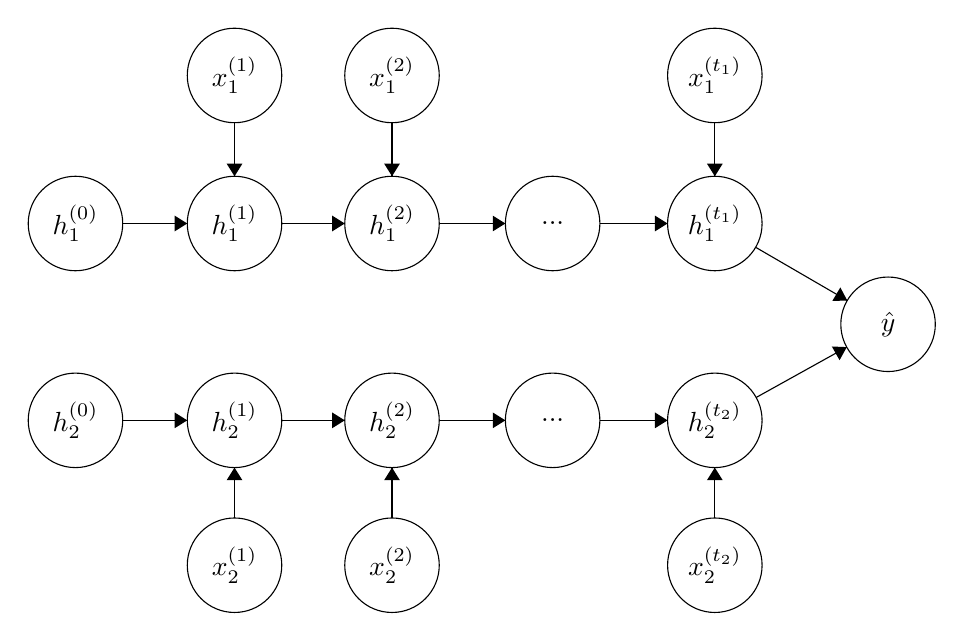
\begin{tikzpicture}[scale=0.2]
\tikzstyle{every node}+=[inner sep=0pt]
\draw [black] (17,-14.5) circle (3);
\draw (17,-14.5) node {$h_1^{(1)}$};
\draw [black] (17,-5.1) circle (3);
\draw (17,-5.1) node {$x_1^{(1)}$};
\draw [black] (27,-14.5) circle (3);
\draw (27,-14.5) node {$h_1^{(2)}$};
\draw [black] (6.9,-14.5) circle (3);
\draw (6.9,-14.5) node {$h_1^{(0)}$};
\draw [black] (27,-5.1) circle (3);
\draw (27,-5.1) node {$x_1^{(2)}$};
\draw [black] (37.2,-14.5) circle (3);
\draw (37.2,-14.5) node {$...$};
\draw [black] (47.5,-14.5) circle (3);
\draw (47.5,-14.5) node {$h_1^{(t_1)}$};
\draw [black] (47.5,-5.1) circle (3);
\draw (47.5,-5.1) node {$x_1^{(t_1)}$};
\draw [black] (6.9,-27) circle (3);
\draw (6.9,-27) node {$h_2^{(0)}$};
\draw [black] (17,-27) circle (3);
\draw (17,-27) node {$h_2^{(1)}$};
\draw [black] (27,-27) circle (3);
\draw (27,-27) node {$h_2^{(2)}$};
\draw [black] (37.2,-27) circle (3);
\draw (37.2,-27) node {$...$};
\draw [black] (47.5,-27) circle (3);
\draw (47.5,-27) node {$h_2^{(t_2)}$};
\draw [black] (17,-36.2) circle (3);
\draw (17,-36.2) node {$x_2^{(1)}$};
\draw [black] (27,-36.2) circle (3);
\draw (27,-36.2) node {$x_2^{(2)}$};
\draw [black] (47.5,-36.2) circle (3);
\draw (47.5,-36.2) node {$x_2^{(t_2)}$};
\draw [black] (58.5,-20.9) circle (3);
\draw (58.5,-20.9) node {$\hat{y}$};
\draw [black] (9.9,-14.5) -- (14,-14.5);
\fill [black] (14,-14.5) -- (13.2,-14) -- (13.2,-15);
\draw [black] (17,-8.1) -- (17,-11.5);
\fill [black] (17,-11.5) -- (17.5,-10.7) -- (16.5,-10.7);
\draw [black] (9.9,-27) -- (14,-27);
\fill [black] (14,-27) -- (13.2,-26.5) -- (13.2,-27.5);
\draw [black] (27,-8.1) -- (27,-11.5);
\fill [black] (27,-11.5) -- (27.5,-10.7) -- (26.5,-10.7);
\draw [black] (30,-14.5) -- (34.2,-14.5);
\fill [black] (34.2,-14.5) -- (33.4,-14) -- (33.4,-15);
\draw [black] (20,-14.5) -- (24,-14.5);
\fill [black] (24,-14.5) -- (23.2,-14) -- (23.2,-15);
\draw [black] (40.2,-14.5) -- (44.5,-14.5);
\fill [black] (44.5,-14.5) -- (43.7,-14) -- (43.7,-15);
\draw [black] (47.5,-8.1) -- (47.5,-11.5);
\fill [black] (47.5,-11.5) -- (48,-10.7) -- (47,-10.7);
\draw [black] (50.09,-16.01) -- (55.91,-19.39);
\fill [black] (55.91,-19.39) -- (55.47,-18.56) -- (54.96,-19.42);
\draw [black] (50.12,-25.55) -- (55.88,-22.35);
\fill [black] (55.88,-22.35) -- (54.93,-22.31) -- (55.42,-23.18);
\draw [black] (47.5,-33.2) -- (47.5,-30);
\fill [black] (47.5,-30) -- (47,-30.8) -- (48,-30.8);
\draw [black] (17,-33.2) -- (17,-30);
\fill [black] (17,-30) -- (16.5,-30.8) -- (17.5,-30.8);
\draw [black] (20,-27) -- (24,-27);
\fill [black] (24,-27) -- (23.2,-26.5) -- (23.2,-27.5);
\draw [black] (27,-33.2) -- (27,-30);
\fill [black] (27,-30) -- (26.5,-30.8) -- (27.5,-30.8);
\draw [black] (30,-27) -- (34.2,-27);
\fill [black] (34.2,-27) -- (33.4,-26.5) -- (33.4,-27.5);
\draw [black] (40.2,-27) -- (44.5,-27);
\fill [black] (44.5,-27) -- (43.7,-26.5) -- (43.7,-27.5);
\end{tikzpicture}
\end{center}
The majority of the algorithms we will try will have this general layout; however, we also plan to try to incorporate features from the other question in the pair in each of the final hidden vectors before making a prediction. We also plan to try augmenting our dataset by creating more non-duplicate pairs of questions by combining different lines of the existing dataset.

\section{Related Work}
Detecting semantically equivalent sentences or questions has been a long-standing problem in natural language processing and understanding. In recent years, the application of deep learning to this problem have offered significant improvements over traditional machine learning methods. Bogdanova et al.[1] found that their convolutional neural network algorithm was more effective than the traditional methods of using Jaccard similarity or support vector machiness in determining whether two questions are duplicates. Sanborn and Skryzalin [3] compared the use of recurrent neural networks and recursive neural networks with traditional machine learning methods and found that recurrent neural networks performed the best on the SemEval-2015 dataset. Their recurrent neural network algorithm will serve as a model for our algorithms in this project. Dey et al. [2] studied alternative methods other than deep learning to approach this problem, arguing that deep learning has inherent flaws that make it unsuitable for detecting semantic similarity. We will use these results to help refine our model beyond the current prevaling models for semantic similarity detection.

\section{Evaluation Plan}
Since our dataset is entirely labeled and has enough data to split into a training set and a test set, we will evaluate the effectiveness of our models by testing its success (\% correctly labeled) on a predesignated test set. We expect to have tables of results with the percentage of correctly labeled pairs for each algorithm we use. We also expect to create confusion matrices for the algorithms to analyze what flaws our models have.

\section{References}
[1] Bogdanova, D., Santos, C.D., Barbosa, L., \& Zadrozny, B. (2015) Detecting semantically equivalent questions in online user forums. {\it Conference on Computational Language Learning}. {\bf 19}: 123-131.\newline
[2] Dey, K., Shrivastava, R. \& Kaushik, S. (2016) A paraphrase and semantic similarity detection system for user generated short-text content on microblogs. {\it International Conference on Computational Linguistics: Technical Papers}, {\bf 16}: 2880-2890.\newline
[3] Sanborn, A. \& Skryzalin, J. (2015) Deep learning for semantic similarity. {\it CS 224d: Deep Learning for Natural Language Processing.} Stanford, CA.
\end{document}

